212. \begin{figure}[ht!]
\center{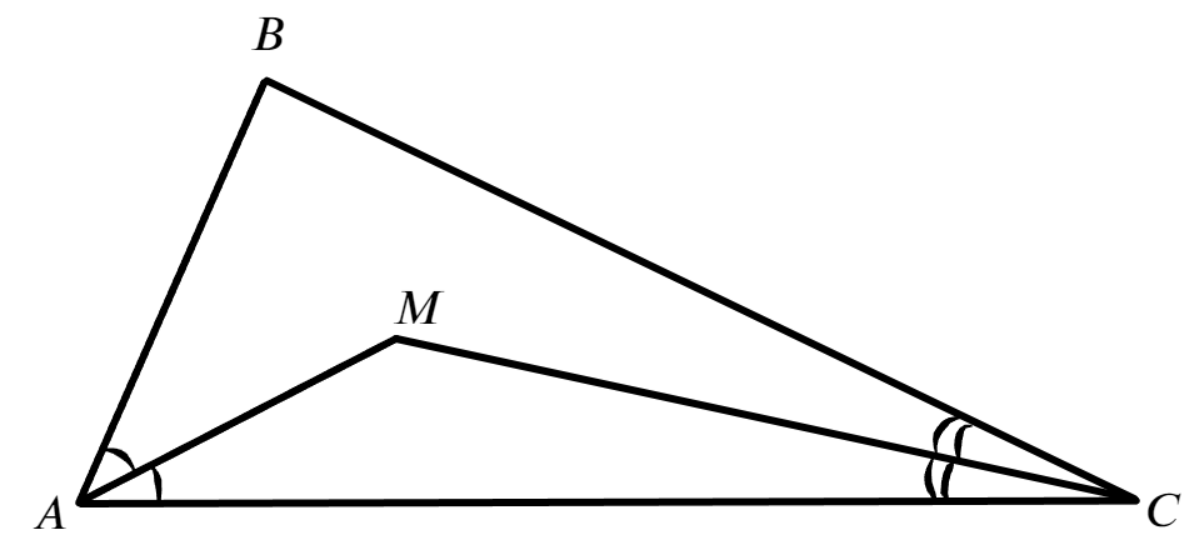
\includegraphics[scale=0.35]{g8-211.png}}
\end{figure}\\
Найдём $\angle AMC=180^\circ-\angle MAC-\angle MCA=180^\circ-\cfrac{1}{2}\left(\angle A +\angle C\right)=180^\circ-\cfrac{1}{2}\left(180^\circ-100^\circ\right)=140^\circ.$ Так как углом между прямыми по определению является острый (или прямой) угол, ответом является $180^\circ-140^\circ=40^\circ.$\\
